\chapter{Result }
\label{ch:intro}

\section{Experimental Environment}

\subsection{Hardware Setup}
All experiments were conducted on a development laptop equipped with an AMD Ryzen™ 7 7735HS processor, 32 GB of DDR5 RAM, and an NVIDIA GPU for accelerated computation , as well as on a \emph{Hunter} mobile robotic platform for on-campus data collection.The robot is equipped with a suite of sensors, including a 3D LiDAR sensor for environment perception, an Inertial Measurement Unit (IMU) for estimating motion and orientation, and a camera for visual reference. An onboard NVIDIA CPU/GPU computing module provides local processing capability.

\begin{figure}[H]
	\centering
	\begin{minipage}{0.5\textwidth}
		\centering
		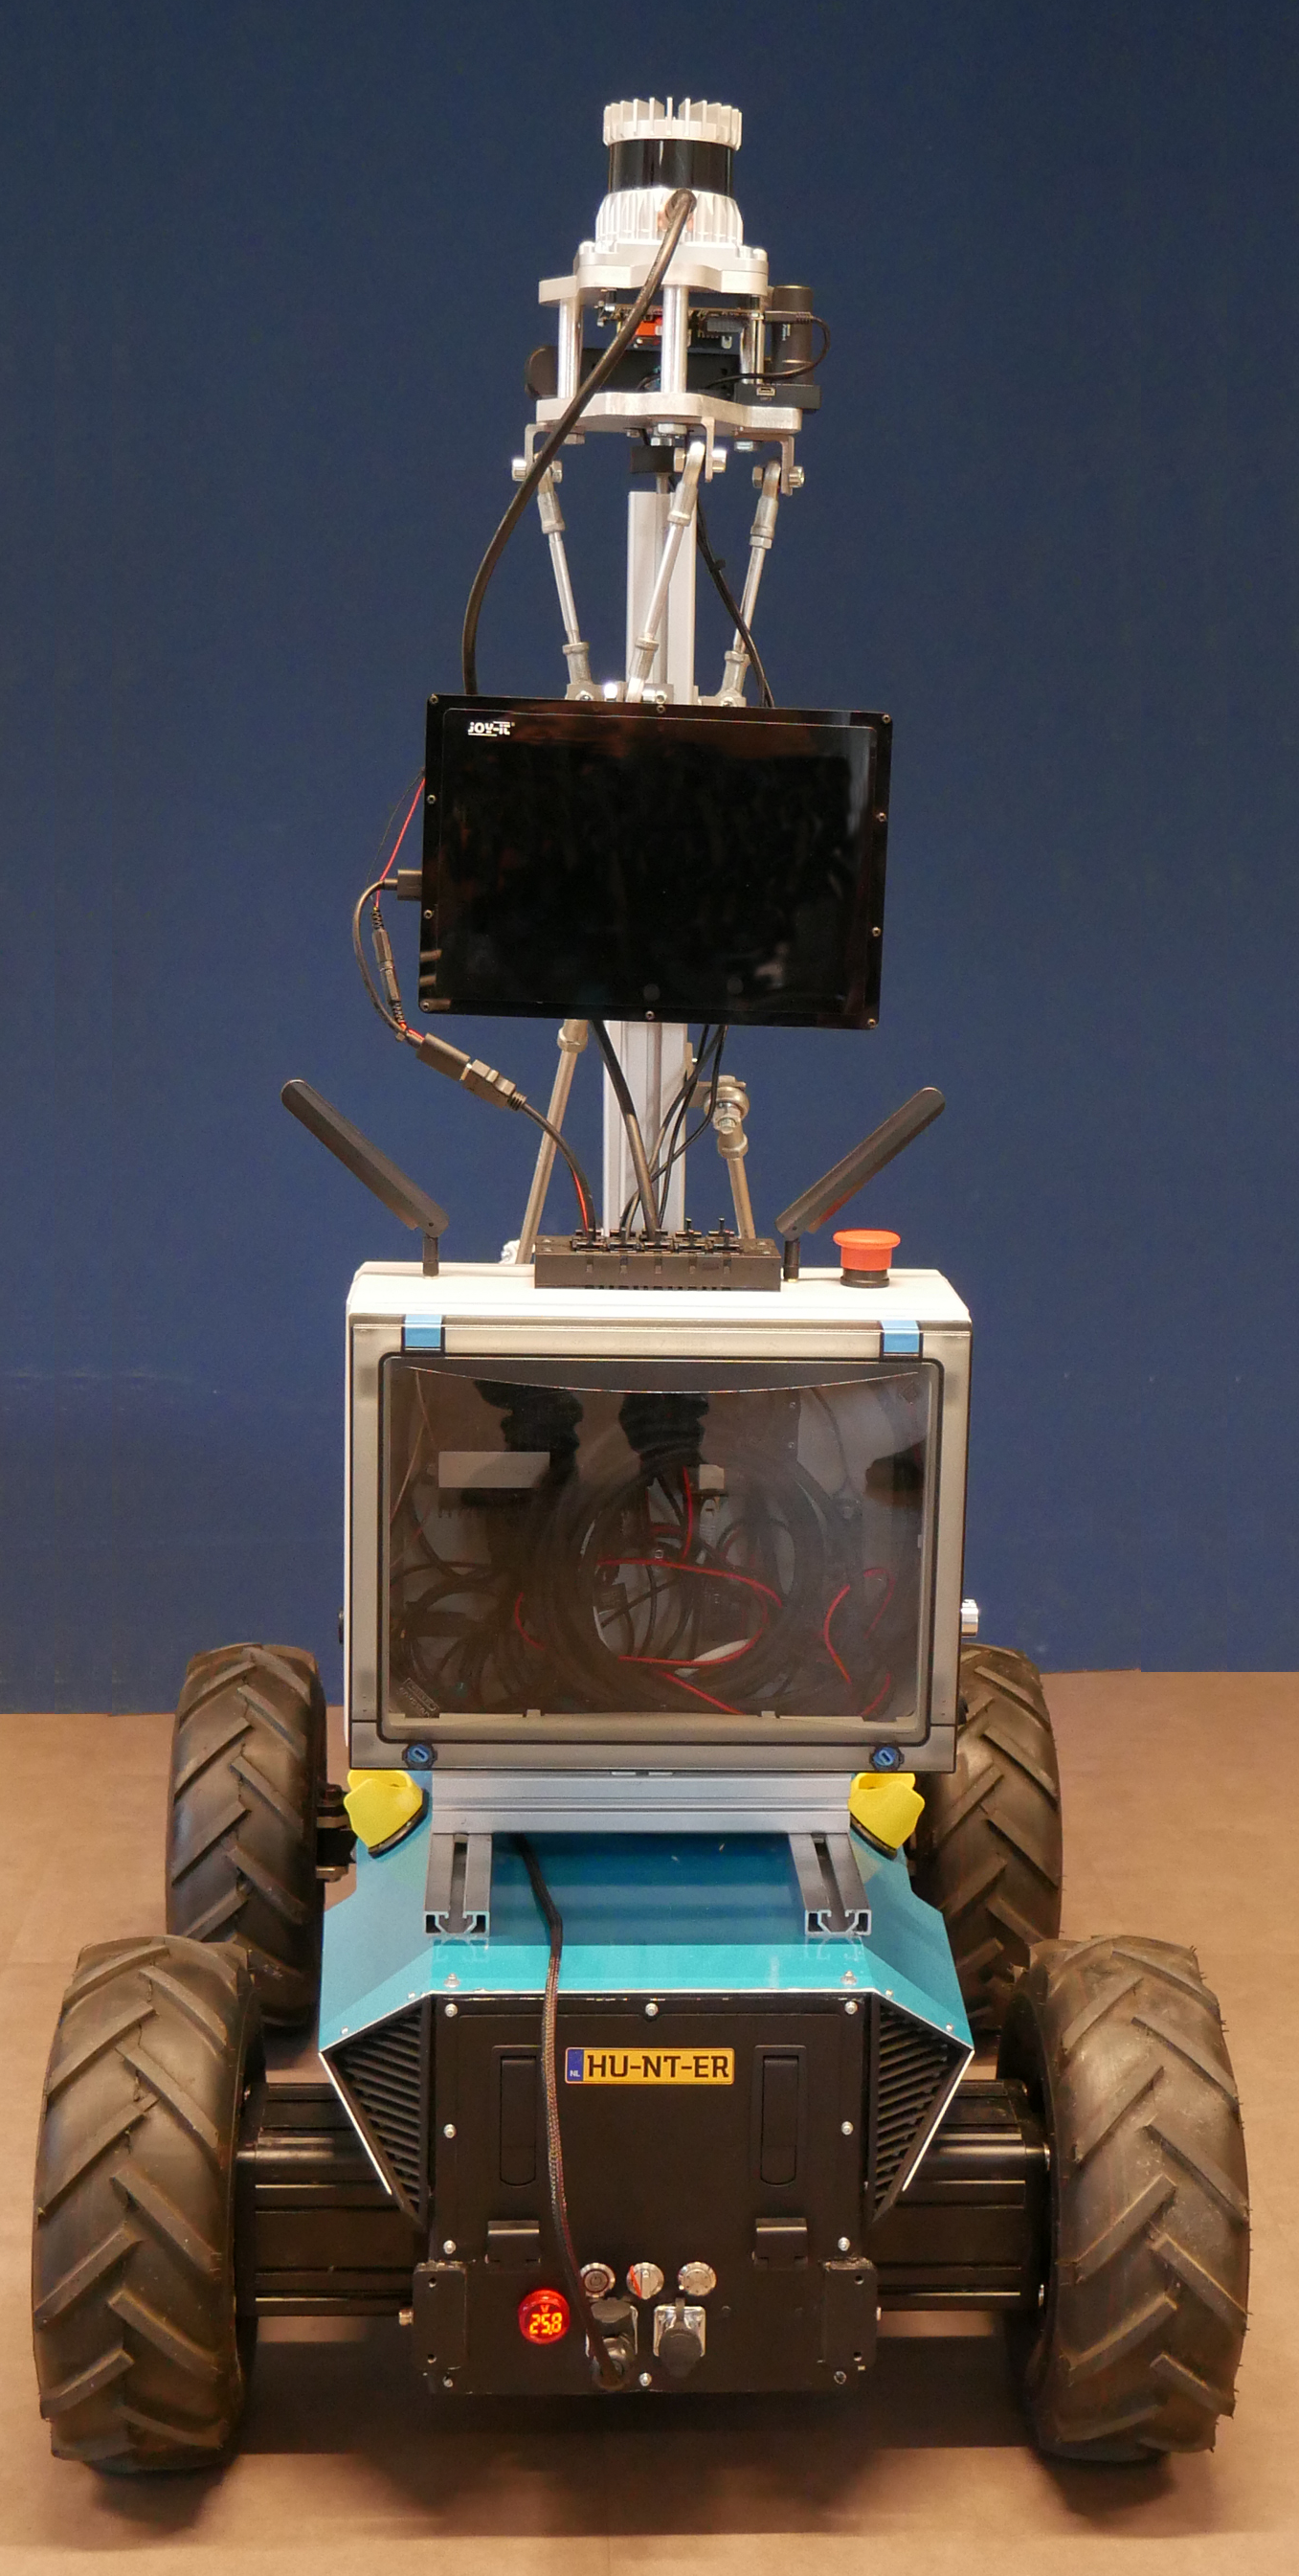
\includegraphics[height=9cm , width=6cm]{images/Hunter_body.png}
		\caption*{(a) Hunter mobile robot platform}
	\end{minipage}\hfill
	\begin{minipage}{0.5\textwidth}
		\centering
		\includegraphics[height=9cm , width=6cm]{images/Hunter_sensor.png}
		\caption*{(b) Sensor configuration (LiDAR, IMU, Camera)}
	\end{minipage}
	\caption{Hardware setup used for real-world data collection and testing: (a) Hunter robotic platform; (b) onboard sensors.}
	\label{fig:hunter-robot-setup}
\end{figure}


\subsection{Software Setup}
Our approach is implemented primarily in C++ on top of the ROS\,2 Humble middleware. We rely on:
\begin{itemize}
  \item \textbf{PCL (Point Cloud Library):} for point cloud data structures and filtering.
  \item \textbf{Eigen:} for linear algebra operations (transformations, matrix computations).
  \item \textbf{ROS\,2 Bag Files:} each dataset is provided or recorded in a \texttt{.bag} format, facilitating playback of sensor data.
\end{itemize}
Additional scripts in Python were employed for plotting and minor data manipulations.

\subsection{Datasets}
We evaluated our map-based localization on multiple datasets, each of which offers LiDAR and IMU data. Table~\ref{tab:datasets} summarizes their key characteristics.

\begin{table}[htbp]
	\centering
	\caption{Overview of datasets and sensor configurations. (L: LiDAR; I: IMU)}
	\label{tab:datasets}
	\resizebox{\textwidth}{!}{%
	\begin{tabular}{lccccc}
	\toprule
	\textbf{Dataset} & \textbf{Seq.} & \textbf{Sensors} & \textbf{LiDAR Type} & \textbf{Frequencies (Hz)} & \textbf{Map Prep. Method} \\
	\midrule
	\textbf{KITTI Odometry} & 05 & L + I & Velodyne HDL-64E & L: 10, I: 100 & GT-based aggregation \\
	%\textbf{KITTI Odometry} & 09 & L + I & Velodyne HDL-64E & L: 10, I: 100 & GT-based aggregation \\
	\textbf{MulRan}         & KiAST-02,03 & L + I & Ouster OS1-64    & L: 10, I: 100 & Fast-LIO2 SLAM \\
	\textbf{Saxion campus}  & seq1,2,3 & L + I & Ouster OS1-128    & L: 10, I: 100 & Fast-LIO2 SLAM \\
	
	\bottomrule
	\end{tabular}%
	}
\end{table}

\paragraph{KITTI Sequences}
We tested on sequences 05 from the KITTI odometry benchmark. These sequences contain semi-urban driving scenarios with moderate speeds. Each frame is timestamped and stored in a ROS\,2 bag for convenient playback.

\paragraph{MulRan (KiAST) Sequences}
Two sequences (KiAST-02, KiAST-03) from the MulRan dataset were used. These contain Ouster OS1-64 LiDAR and IMU measurements in campus-like settings with dynamic objects and complex geometry. The ROS\,2 bags allow consistent replay for algorithm testing.

\subsection{Map Preparation}
For each dataset, a prior 3D map was generated before running the localization:

\begin{itemize}
    \item \textbf{KITTI:} We leveraged the official ground-truth poses to transform and aggregate each LiDAR frame into a global coordinate system. The resulting dense point cloud was lightly downsampled (e.g., voxel size of 0.1\,m).
    \item \textbf{MulRan (KiAST) and Campus (Saxion) Dataset:} No direct ground truth was provided, so we employed \textit{Fast-LIO2 SLAM} to build a consistent map from repeated traversals. This method fuses LiDAR scans and IMU data for robust odometry. The final aggregated map was also voxel-downsampled.
\end{itemize}

In both cases, the final global point cloud is subdivided into manageable tiles for efficient dynamic loading during localization. Each tile is stored as a separate file or database entry keyed by tile coordinates, allowing the system to load only relevant tiles based on the vehicle’s current estimated position.

Overall, this setup ensures that the offline map is readily available in a lightweight format, and the runtime memory footprint remains controlled as the vehicle traverses large-scale environments.


\section{Performance Evaluation}
This section presents the experimental results evaluating the proposed LiDAR-inertial localization system. The evaluation is divided into two main parts: performance under standard conditions, and extended experiments conducted under challenging scenarios to assess system robustness. Standard conditions refer to environments where the reference map is up-to-date, sensor data is relatively noise-free, and dynamic objects are present but not explicitly removed. In contrast, the challenging scenarios include environments with high dynamic object density, transitions between mapped and unmapped regions, low-feature boundary zones, and long-term variations such as map aging.
\subsection{ Localization Performance in Standard Conditions}

\subsubsection{Saxion Campus Dataset}
We evaluated our proposed LiDAR-inertial localization system on three sequences collected from the Saxion campus, representing short, medium, and long trajectories with varying coverage areas and trajectory complexity.Quantitative performance is assessed using Absolute Pose Error (APE) and rotational error after SE(3) alignment.

 Table \ref{tab:ape_rot_saxion_seq1} , \ref{tab:ape_rot_saxion_seq2} , \ref{tab:ape_rot_saxion_seq3} summarize translation and rotation error statistics, including maximum, mean, and RMSE values for the three Saxion sequences. The results show that the proposed system consistently yields lower errors compared to its baseline component Fast-LIO odometry and low frequency NDT-based map matching. 



\begin{table}[H]
	\centering
	\renewcommand{\arraystretch}{0.6}
	\setlength{\tabcolsep}{15pt}
	\caption{Translation (APE) and Rotation Error statistics for Saxion \textbf{Sequence 1} }
	\label{tab:ape_rot_saxion_seq1}
	
	\begin{adjustbox}{width=\textwidth}
		\begin{tabular}{@{}lccccccc@{}}
			\toprule
			\textbf{Method} & \textbf{Metric} & \textbf{Max} & \textbf{Mean} & \textbf{Median} & \textbf{Min} & \textbf{RMSE} & \textbf{Std Dev} \\
			\midrule
			
			\multirow{2}{*}{\textbf{Proposed (Fusion)}} 
			& APE (m)        & 0.395   & \textbf{0.052 }   & \textbf{0.041}     & \textbf{0.003 }   &\textbf{ 0.067}   & \textbf{0.042 }\\
			& Rot. (deg)     & \textbf{4.715}   & \textbf{0.321}    & \textbf{0.169}     &\textbf{ 0.030 }   & \textbf{0.583}   &\textbf{ 0.486} \\
			\midrule
			
			\multirow{2}{*}{NDT Scan Matching} 
			& APE (m)        & \textbf{0.363 }  & 0.074    & 0.067     & 0.012    & 0.084   & \textbf{0.041} \\
			& Rot. (deg)     & 5.832   & 0.503    & 0.299     &\textbf{ 0.012}    & 0.813   & 0.639 \\
			\midrule
			
			\multirow{2}{*}{Fast-LIO} 
			& APE (m)        & 7.594   & 1.456    & 0.933     & 0.322    & 2.197   & 1.645 \\
			& Rot. (deg)     & 6.213   & 1.631    & 1.304     & 0.419    & 2.072   & 1.278 \\
			\bottomrule
		\end{tabular}
	\end{adjustbox}
\end{table}

\begin{figure}[H]
	\centering
	\begin{tikzpicture}
		
		% Main trajectory image
		\node[anchor=south west, inner sep=0] (main) at (0,0)
		{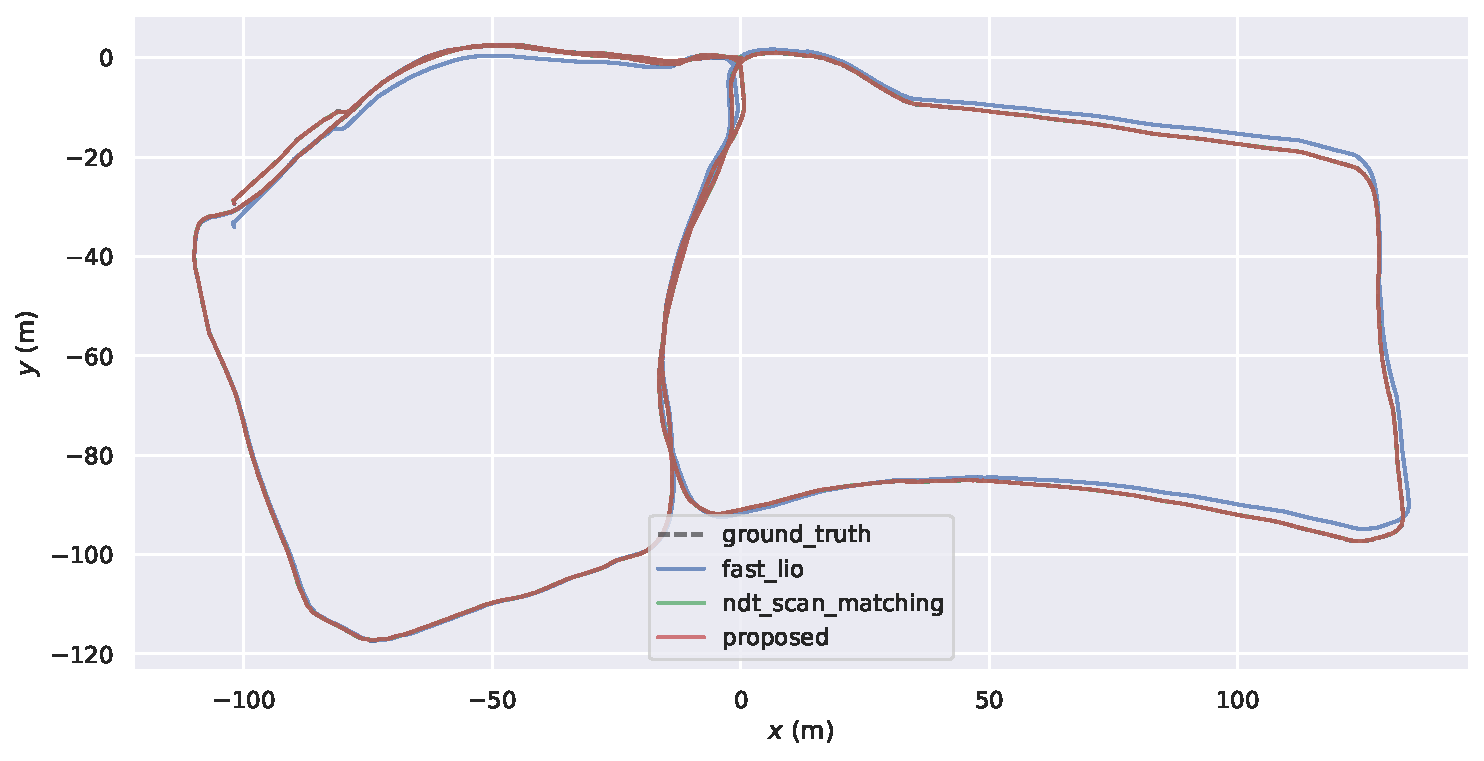
\includegraphics[width=0.9\textwidth]{images/trajectory_plot_seq1.pdf}};
		% Coordinate system normalized to the image
		\begin{scope}[x={(main.south east)}, y={(main.north west)}]
			% Red dashed rectangle for zoom box (adjust coordinates!)
			\draw[red, thick, dashed] (0.85, 0.20) rectangle (0.98, 0.45);
			% Red arrow from zoom box to zoomed-in image
			\draw[->, red, thick] (0.98, 0.45) -- (1, 0.85);
		\end{scope}
		
		% Zoomed-in image overlay (use exact x/y in cm to place)
		\node[anchor=south west] at (8, 6)
		{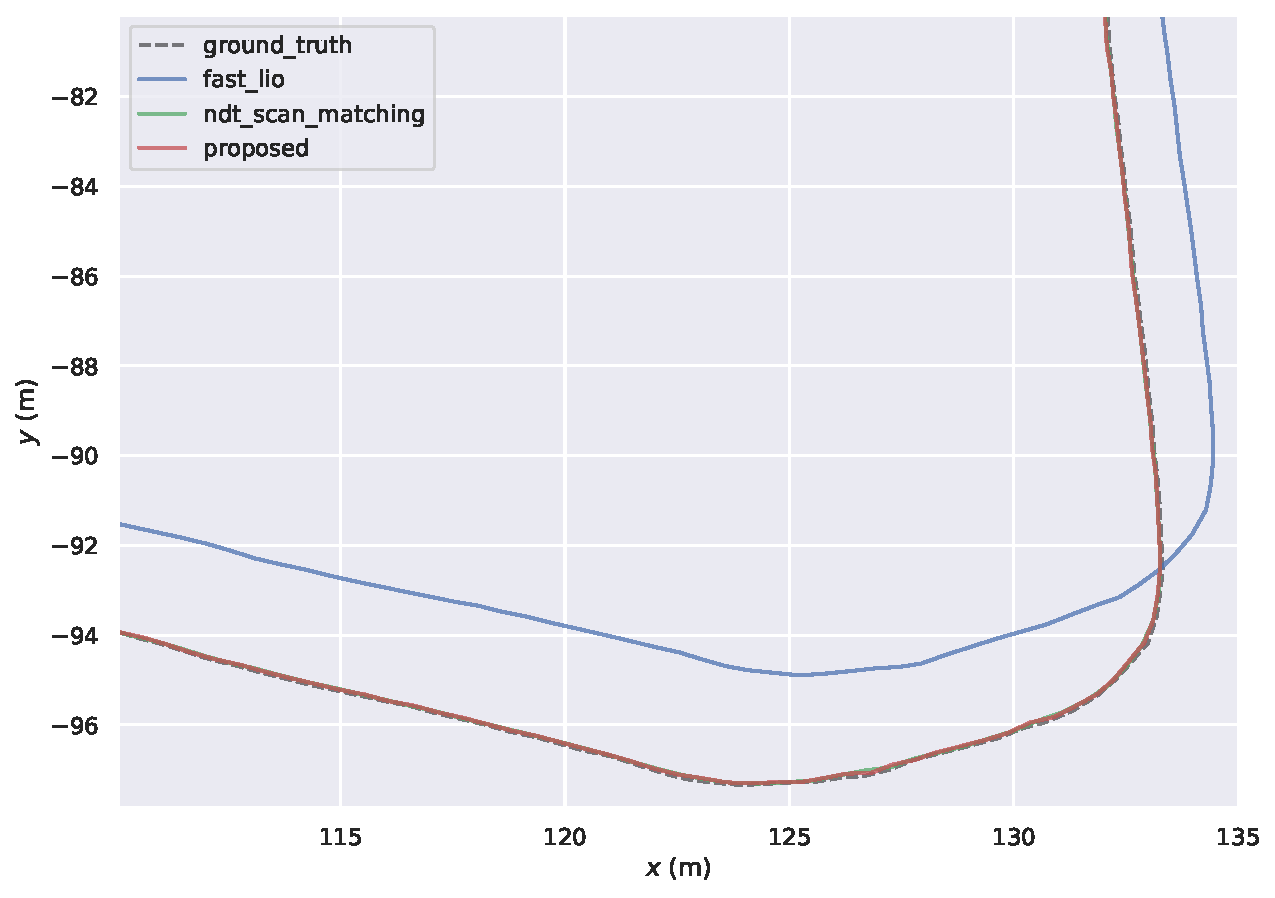
\includegraphics[width=0.5\textwidth]{images/trajectory_zoom_seq1.pdf}};
		
		% Optional label
		%\node at (15, 4.6) {\small Zoomed-in detail};
		
	\end{tikzpicture}
	\caption[Saxion Sequence 01 – Trajectory Alignment with Zoomed Comparison]%
	{\textbf{Saxion Sequence 01 – Trajectory Alignment.} 
		The figure shows the estimated trajectories from FAST-LIO2, low frequency NDT map matching , and the proposed method, overlaid against ground truth. The red dashed box indicates the zoomed region.
	}
	\label{fig:saxion-seq1-trajectory-zoom}
	
\end{figure}


\begin{table}[H]
	\centering
	\renewcommand{\arraystretch}{0.6}
	\setlength{\tabcolsep}{15pt}
	\caption{Translation (APE) and Rotation Error statistics for Saxion \textbf{Sequence 2} }
	\label{tab:ape_rot_saxion_seq2}
	
	\begin{adjustbox}{width=\textwidth}
		\begin{tabular}{@{}lccccccc@{}}
			\toprule
			\textbf{Method} & \textbf{Metric} & \textbf{Max} & \textbf{Mean} & \textbf{Median} & \textbf{Min} & \textbf{RMSE} & \textbf{Std Dev} \\
			\midrule
			
			\multirow{2}{*}{\textbf{Proposed (Fusion)}} 
			& APE (m)        & 0.440   & \textbf{0.090}   & \textbf{0.075}     & \textbf{0.005}   & \textbf{0.107}   & \textbf{0.058} \\
			& Rot. (deg)     & 4.356   & \textbf{0.782}   & \textbf{0.539}     & \textbf{0.051}   & \textbf{1.046}   & \textbf{0.695} \\
			\midrule
			
			\multirow{2}{*}{NDT Scan Matching} 
			& APE (m)        & \textbf{0.245}   & 0.102   & 0.094     & 0.009    & 0.118   & 0.059 \\
			& Rot. (deg)     & \textbf{2.639}   & 1.195   & 1.127     & 0.103    & 1.393   & 0.715 \\
			\midrule
			
			\multirow{2}{*}{Fast-LIO} 
			& APE (m)        & 9.467   & 2.507   & 1.944     & 0.370    & 3.301   & 2.147 \\
			& Rot. (deg)     & 5.494   & 2.250   & 1.568     & 0.202    & 2.680   & 1.456 \\
			\bottomrule
		\end{tabular}
	\end{adjustbox}
\end{table}

\begin{figure}[H]
	\centering
	\begin{tikzpicture}
		
		% Main trajectory image
		\node[anchor=south west, inner sep=0] (main) at (0,0)
		{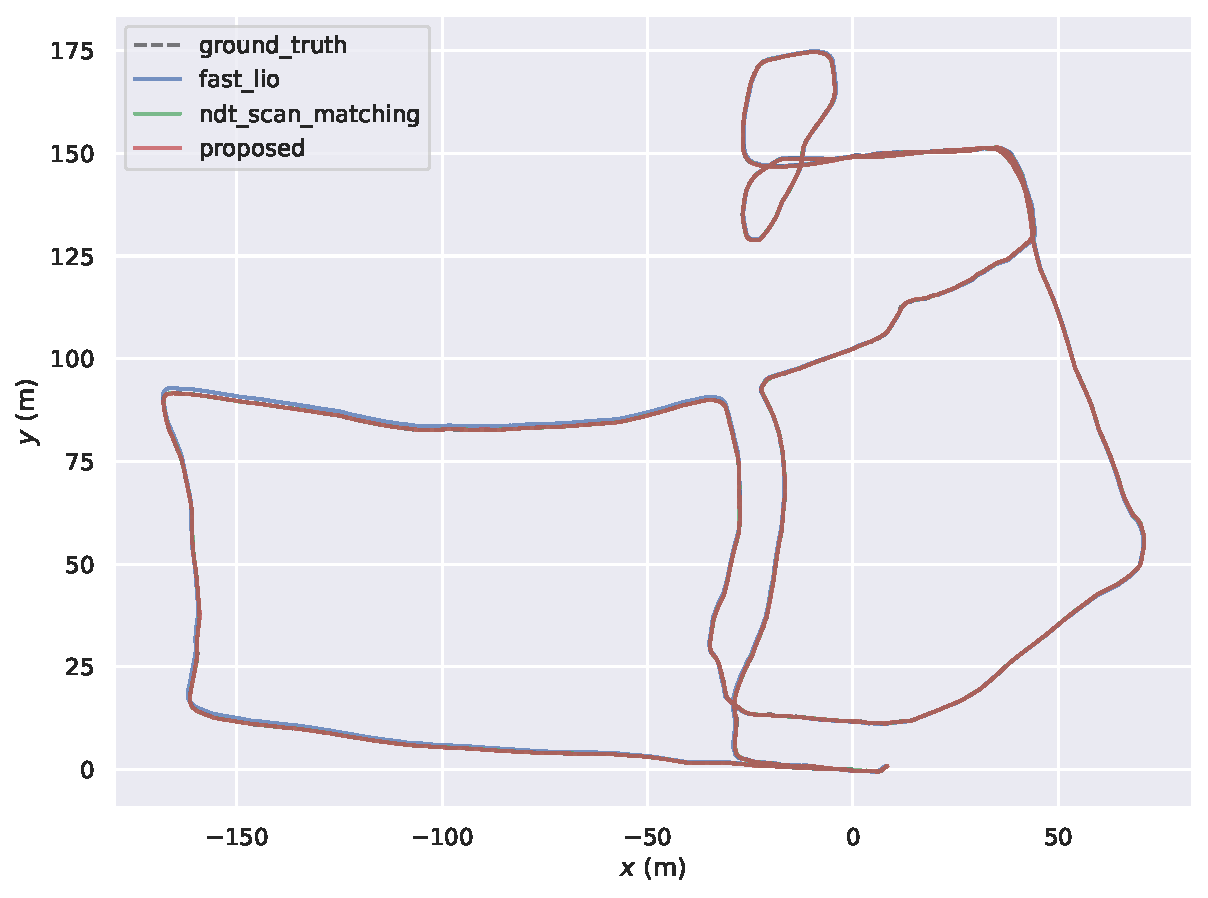
\includegraphics[width=1\textwidth]{images/trajectory_plot_seq2.pdf}};
		% Coordinate system normalized to the image
		\begin{scope}[x={(main.south east)}, y={(main.north west)}]
			% Red dashed rectangle for zoom box (adjust coordinates!)
			\draw[red, thick, dashed] (0.1, 0.45) rectangle (0.25, 0.6);
			% Red arrow from zoom box to zoomed-in image
			\draw[->, red, thick] (0.25, 0.6) -- (.265, 0.65);
		\end{scope}
		
		% Zoomed-in image overlay (use exact x/y in cm to place)
		\node[anchor=south west] at (3.9, 6.2)
		{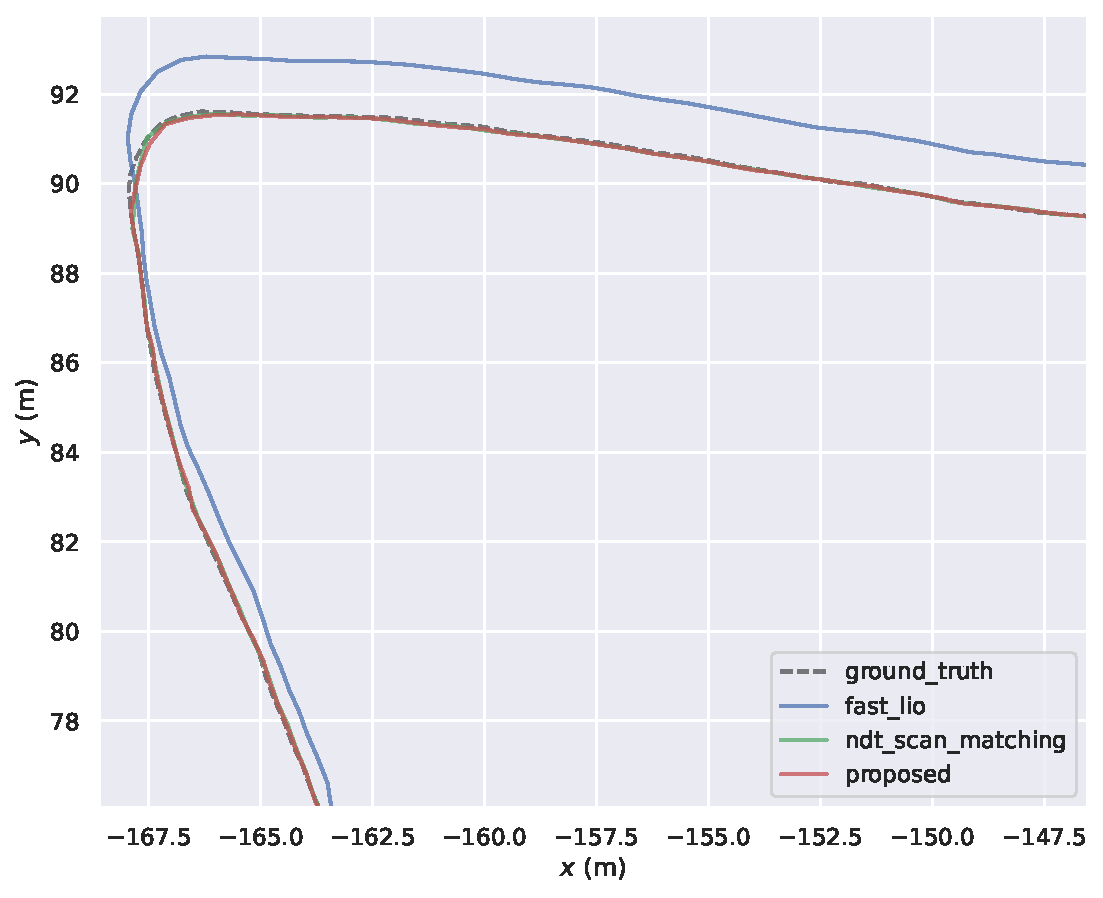
\includegraphics[width=0.34\textwidth]{images/trajectory_plot_zoom_seq2.pdf}};
		
		% Optional label
		%\node at (15, 4.6) {\small Zoomed-in detail};
		
	\end{tikzpicture}
	\caption[Saxion Sequence 02– Trajectory Alignment with Zoomed Comparison]%
	{\textbf{Saxion Sequence 02 – Trajectory Alignment.} 
		The figure shows the estimated trajectories from FAST-LIO2, low frequency NDT map matching , and the proposed method, overlaid against ground truth. The red dashed box indicates the zoomed region.
	}
	\label{fig:saxion-seq2-trajectory-zoom}
	

\end{figure}

\begin{table}[H]
	\centering
	\renewcommand{\arraystretch}{0.6}
	\setlength{\tabcolsep}{15pt}
	\caption{Translation (APE) and Rotation Error statistics for Saxion \textbf{Sequence 3} }
	\label{tab:ape_rot_saxion_seq3}
	
	\begin{adjustbox}{width=\textwidth}
		\begin{tabular}{@{}lccccccc@{}}
			\toprule
			\textbf{Method} & \textbf{Metric} & \textbf{Max} & \textbf{Mean} & \textbf{Median} & \textbf{Min} & \textbf{RMSE} & \textbf{Std Dev} \\
			\midrule
			
			\multirow{2}{*}{\textbf{Proposed (Fusion)}} 
			& APE (m)        & 0.821   & \textbf{0.097}   & \textbf{0.072}     & \textbf{0.004}   & 0.135   & 0.094 \\
			& Rot. (deg)     & 5.016   & \textbf{0.725}   & \textbf{0.472}     & \textbf{0.076}   & \textbf{1.039}   & \textbf{0.743} \\
			\midrule
			
			\multirow{2}{*}{NDT Scan Matching} 
			& APE (m)        & \textbf{0.297}   & 0.113   & 0.100     & 0.025    & \textbf{0.126}   & \textbf{0.056} \\
			& Rot. (deg)     & 3.236   & 1.373   & 1.286     & 0.131    & 1.652   & 0.919 \\
			\midrule
			
			\multirow{2}{*}{Fast-LIO} 
			& APE (m)        & 3.475   & 1.468   & 1.254     & 0.028    & 1.862   & 1.145 \\
			& Rot. (deg)     & 2.750   & 0.955   & 0.953     & 0.069    & 1.088   & 0.522 \\
			\bottomrule
		\end{tabular}
	\end{adjustbox}
\end{table}

\subsubsection{KITTI Dataset} 
To benchmark the proposed system against existing SLAM methods, we evaluated it on KITTI Sequence 05 alongside KISS-ICP and MOLA SLAM. As shown in Table \ref{tab:ape_rot_kitti_seq5}, the proposed method achieves significantly lower translation and rotation errors, attaining decimeter-level accuracy through the incorporation of map-based matching. The trajectory plot Figure \ref{fig:kitti05-traj-zoom} shows that our method closely follows the ground truth throughout the sequence. A zoomed-in view at the end of the trajectory highlights substantial deviations in both KISS-ICP and MOLA SLAM, while the proposed approach remains well-aligned with the reference path.

\begin{table}[H]
	\centering
	\renewcommand{\arraystretch}{0.6}
	\setlength{\tabcolsep}{15pt}
	\caption{Translation (APE) and Rotation Error statistics for \textbf{KITTI Sequence 05}}
	\label{tab:ape_rot_kitti_seq5}
	
	\begin{adjustbox}{width=\textwidth}
		\begin{tabular}{@{}lccccccc@{}}
			\toprule
			\textbf{Method} & \textbf{Metric} & \textbf{Max} & \textbf{Mean} & \textbf{Median} & \textbf{Min} & \textbf{RMSE} & \textbf{Std Dev} \\
			\midrule
			
			\multirow{2}{*}{\textbf{Proposed}} 
			& APE (m)        & \textbf{0.483}   & \textbf{0.121}   & \textbf{0.102}     & \textbf{0.007}   & \textbf{0.143}   & \textbf{0.077} \\
			& Rot. (deg)     & \textbf{1.914}   & \textbf{0.376}   & \textbf{0.356}     & \textbf{0.078}   & \textbf{0.402}   & \textbf{0.144} \\
			\midrule
			
			\multirow{2}{*}{KISS-ICP} 
			& APE (m)        & 5.067   & 1.460   & 1.445     & 0.281    & 1.604   & 0.666 \\
			& Rot. (deg)     & 2.696   & 1.376   & 1.441     & 0.000    & 1.465   & 0.504 \\
			\midrule
			
			\multirow{2}{*}{MOLA SLAM} 
			& APE (m)        & 6.817   & 1.539   & 1.447     & 0.306    & 1.793   & 0.920 \\
			& Rot. (deg)     & 3.861   & 1.931   & 1.886     & 0.000    & 2.015   & 0.577 \\
			\bottomrule
		\end{tabular}
	\end{adjustbox}
\end{table}


\begin{figure}[H]
	\centering
	\begin{tikzpicture}
		
		% Main trajectory image
		\node[anchor=south west, inner sep=0] (main) at (0,0)
		{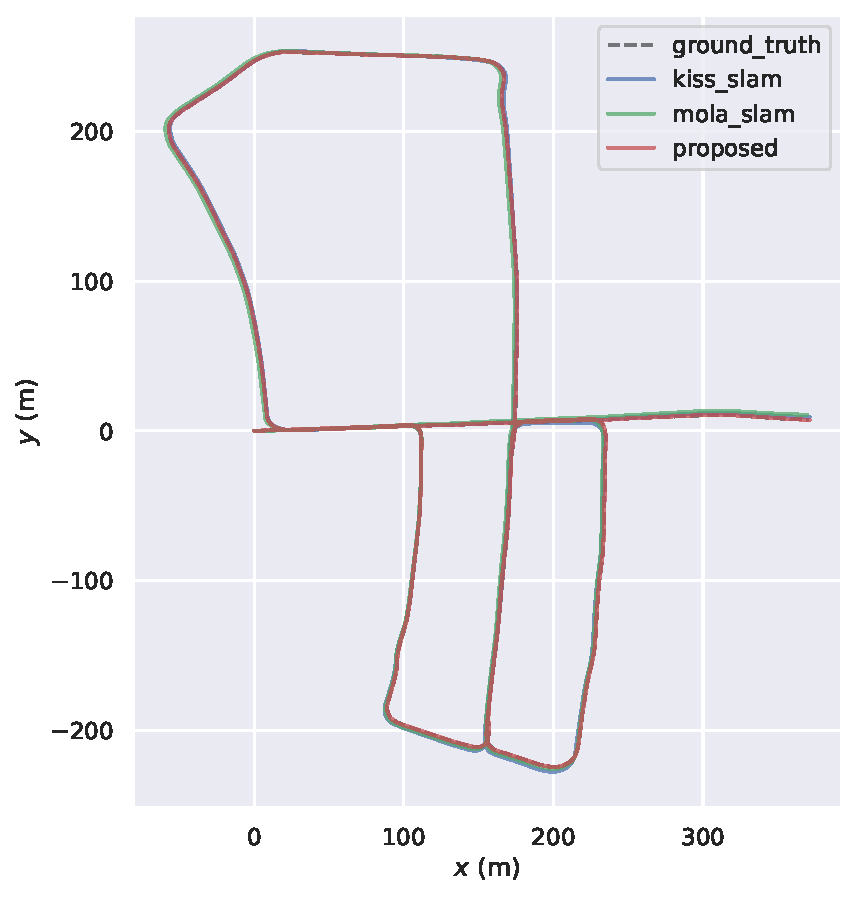
\includegraphics[width=0.8\textwidth]{images/trajectory_plot_kitti.pdf}};
		% Coordinate system normalized to the image
		\begin{scope}[x={(main.south east)}, y={(main.north west)}]
			% Red dashed rectangle for zoom box (adjust coordinates!)
			\draw[red, thick, dashed] (0.85, 0.5) rectangle (0.95, 0.56);
			% Red arrow from zoom box o tzoomed-in image
			\draw[->, red, thick] (0.95, 0.55) -- (0.97, 0.57);
		\end{scope}
		
		% Zoomed-in image overlay (use exact x/y in cm to place)
		\node[anchor=south west] at (8.1, 7)
		{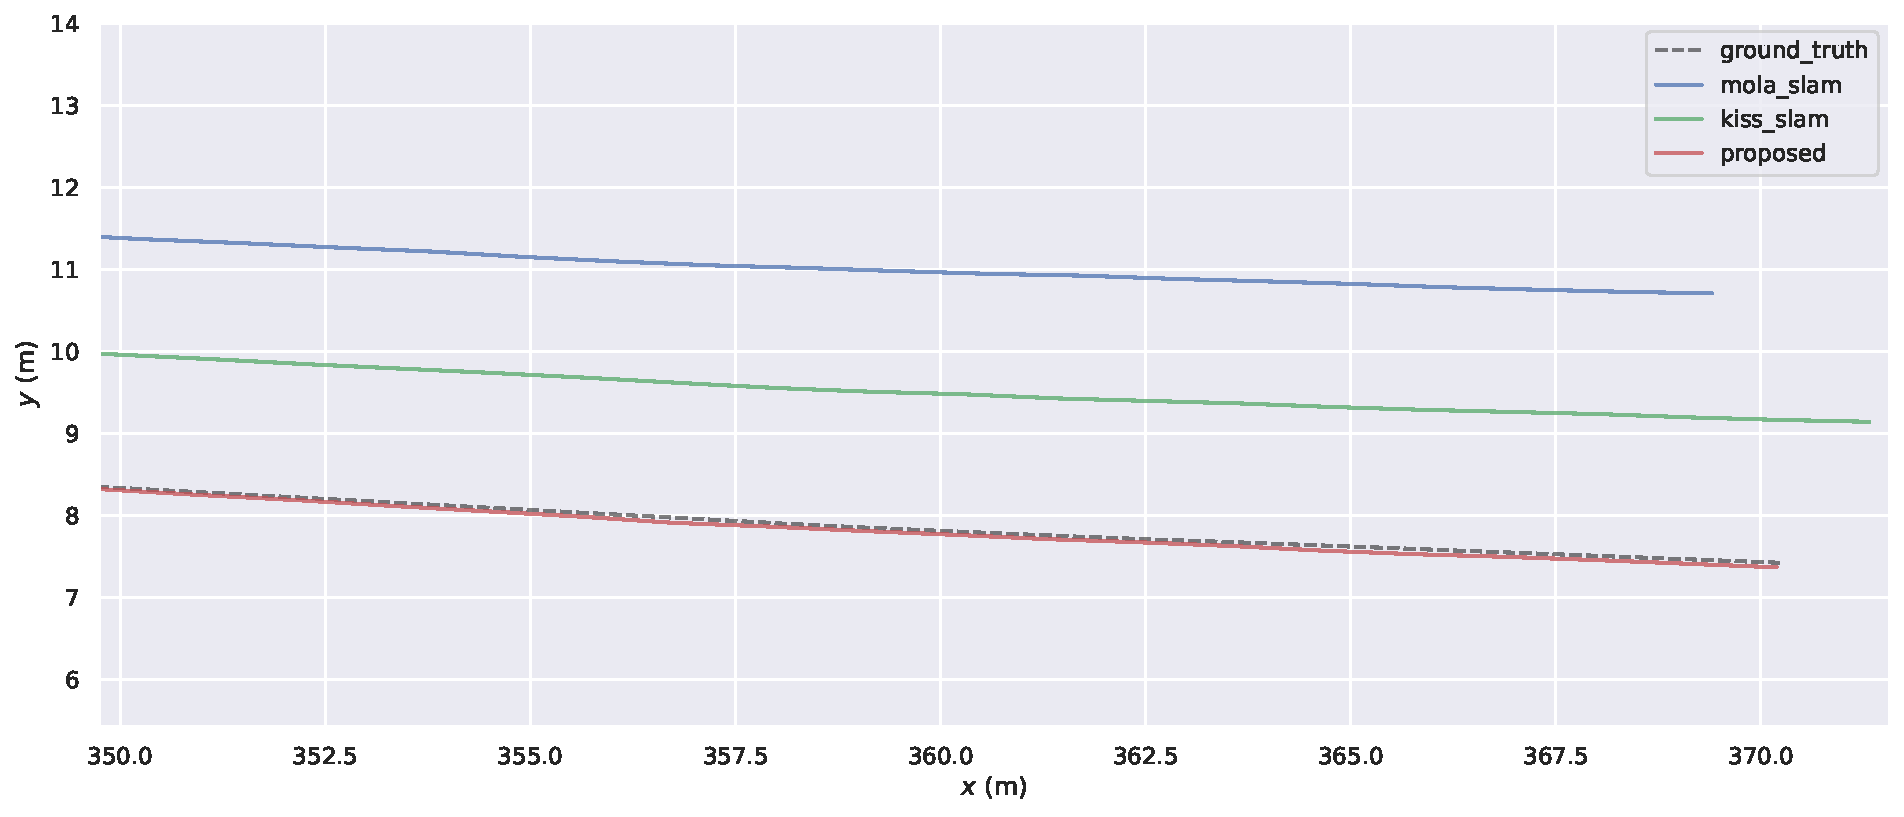
\includegraphics[width=0.5\textwidth]{images/trajectory_plot_kitti_zoom.pdf}};
		
		% Optional label
		%\node at (15, 4.6) {\small Zoomed-in detail};
		
	\end{tikzpicture}
	
	\caption[KITTI Sequence 05 – Trajectory Alignment with Zoomed Comparison]%
	{\textbf{KITTI Sequence 05 – Trajectory Alignment.} 
		The figure shows the estimated trajectories from KISS-SLAM, MOLA SLAM, and the proposed method, overlaid against ground truth.The red dashed box indicates the zoomed region..
	}
	\label{fig:kitti05-traj-zoom}
\end{figure}

\subsection{ Extended Evaluation Under Challenging Conditions}


\subsubsection{Scenario A – Dynamic Object Removal Impact}
Compare localization with vs. without dynamic object filtering

Evaluate:

APE improvement

Stability in dense environments (e.g., parked or moving vehicles)

Visualize retained vs. removed points and their effect on pose drift

\subsubsection{ Scenario B – Unmapped or Transition Zones}
Compare localization with vs. without dynamic object filtering

Evaluate:

APE improvement

Stability in dense environments (e.g., parked or moving vehicles)

Visualize retained vs. removed points and their effect on pose drift

\subsubsection{Scenario C – Low-Feature or Boundary Zones}

Analyze performance in areas with poor LiDAR structure (e.g., open space, flat walls)

Evaluate matching success rate and error spikes

Discuss influence of scan-to-map quality

\subsubsection{Scenario D – Map Aging or Revisit Tests}

    Use old maps (recorded ~1 month earlier)

Assess performance degradation:

Temporal mismatch vs. accuracy

Object layout drift impact (e.g., moved vehicles or structures)




% \subsection{Dynamic Map Loading}
% Dynamic map loading is implemented to optimize memory and computational efficiency in large-scale localization. Instead of loading the entire map, only the relevant portion is loaded dynamically based on the robot’s current position. This method significantly reduces memory consumption and improves real-time performance.
% The following images from **RViz** illustrate the dynamic map loading process. The **active map region** is highlighted in red colors, showing how the system loads only necessary portions as the robot moves.

% \begin{figure}[h]
%     \centering
%     \begin{subfigure}{0.49\textwidth}
%         \includegraphics[width=\linewidth]{images/kitti_load2.png}
%         \caption{Initial Map Loading}
%     \end{subfigure}
%     \hfill
%     \begin{subfigure}{0.49\textwidth}
%         \includegraphics[width=\linewidth]{images/kitti_load1.png}
%         \caption{Map Updated as Robot Moves}
%     \end{subfigure}
    
%     % \begin{subfigure}{0.45\textwidth}
%     %     \includegraphics[width=\linewidth]{map_loading_3.png}
%     %     \caption{Further Update in a New Region}
%     % \end{subfigure}
%     % \hfill
%     % \begin{subfigure}{0.45\textwidth}
%     %     \includegraphics[width=\linewidth]{map_loading_4.png}
%     %     \caption{Final State: Only Active Regions are Loaded}
%     % \end{subfigure}
    
%     \caption{RViz Visualization of Dynamic Map Loading. The red region represents the currently loaded map section and the green color shows current LIDAR scan}
%     \label{fig:dynamic_map_loading}
% \end{figure}

% \subsection{NDT  Localization Result}


% \paragraph{NDT scan and map alignment }
% Figure \ref{fig:ndt_allignment} show the NDT registration visualization in saxion campus dataset.
% \begin{figure}[h]
%     \centering
%     \begin{subfigure}{0.49\textwidth}
%         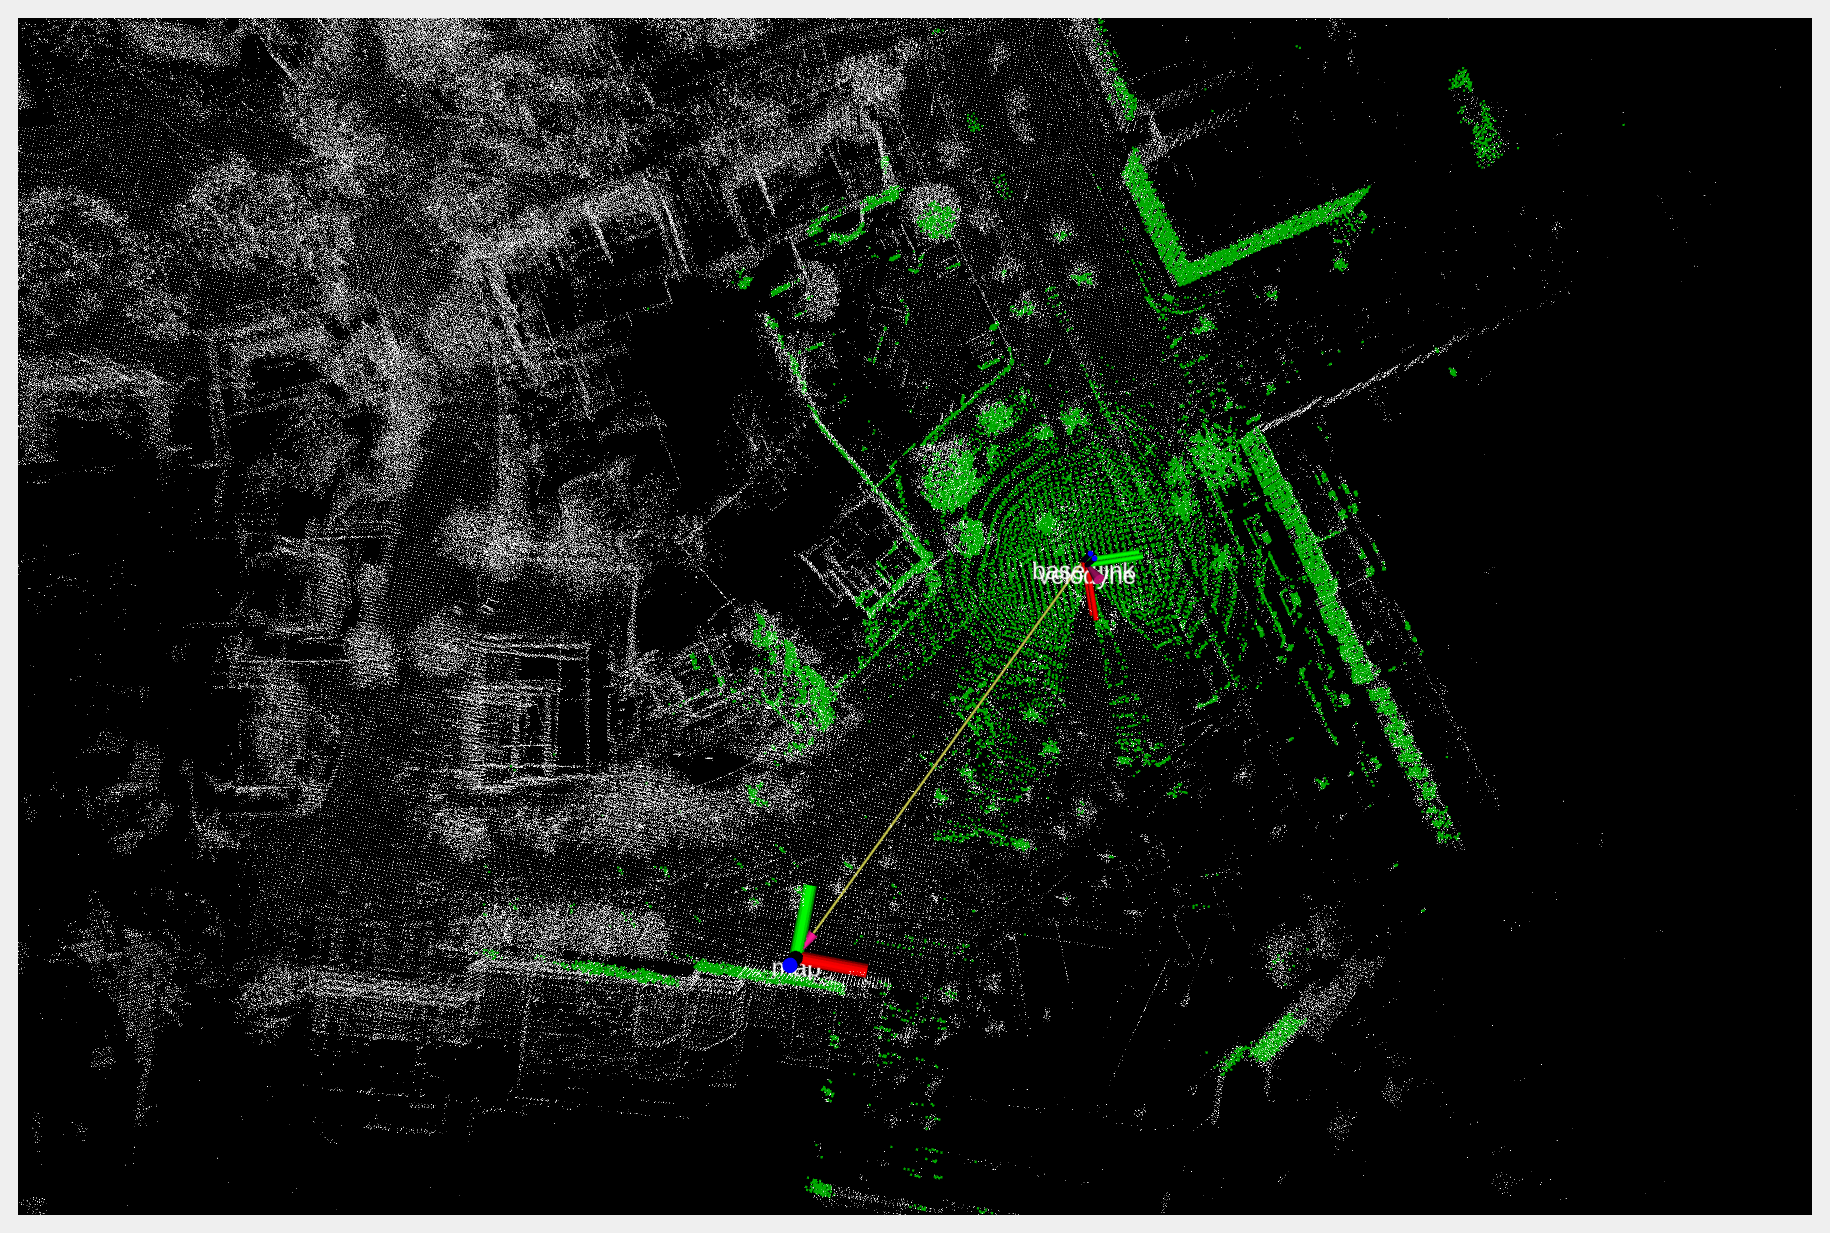
\includegraphics[width=\linewidth]{images/ndt_scan_map_matching2.png}
%         \caption{Initial Map Loading}
%     \end{subfigure}
%     \hfill
%     \begin{subfigure}{0.49\textwidth}
%         \includegraphics[width=\linewidth]{images/ndt_scan_map_matching.png}
%         \caption{Map Updated as Robot Moves}
%     \end{subfigure}
%     \caption{RViz Visualization of current scan with map allignment using NDT registration. The green color scan represents the currently scan and the greycolor  color shows global map}
%     \label{fig:ndt_allignment}
% \end{figure}


% \paragraph{KITTI Sequence 5 Test}
% Multiple runs of NDT localization on KITTI Sequence 5 revealed cases where localization either succeeded or failed. Below, we present separate images for these scenarios.

% \begin{itemize}
%     \item As shown in Figure \ref{fig:kitti_fail}, localization failure occurs in certain sections of the trajectory.
%     \begin{figure}[ht]
%     \centering
%     \includegraphics[width=0.6\textwidth]{images/kitti_failure.png}
%     \caption{Example of NDT localization failure in KITTI Sequence 5.}
%     \label{fig:kitti_fail}
%     \end{figure}

%     \item Figure \ref{fig:kitti_success} shows a scenario where localization performs well. The robot finishes the whole trajectory.
%     \begin{figure}[ht]
%     \centering
%     \includegraphics[width=0.6\textwidth]{images/kitti_suces.png}
%     \caption{Successful NDT localization in KITTI Sequence 5.}
%     \label{fig:kitti_success}
%     \end{figure}

% \end{itemize}

% \paragraph{Saxion Dataset Test}

% \begin{figure}[ht]
%     \centering
%     \includegraphics[width=0.6\textwidth]{images/saxionfailure.png}
%     \caption{Example of NDT localization failure in the Saxion dataset.}
%     \label{fig:saxion_fail}
% \end{figure}

% In Figure \ref{fig:saxion_fail}, NDT localization fails in certain regions of the Saxion dataset.


% \subsubsection{Things to be Checked for Localization failure }
% \begin{itemize}
%     \item NDT registration parameters 
%     \item Map and Scan down-sampling parameter 
%     \item Map Retrial radius 
%     \item Map Quality 
% \end{itemize}
